\addtocontents{toc}{\protect\newpage}

\chapter{Концептуальна модель формальної системи мов}
\epigraph{Присвячується автору першої дисертації з гомотопічноїї теорії типів}{Майклу Уорену}

Другий розділ описує розвиток концептуальної моделі системи доведення теорем як сукупності:
1) категорій, які розкривають семантику конкретної теорії типів (мови програмування) як синтаксису, або є її метатеорією.
2) теорії для маніпуляції мовними синтаксисами та програмами (мовні категорії).
Ця концептуальна модель є сокупністю категорій, що пропонує фреймворк або стандарт
на розробку та формалізацію формальних мов. Усі мови програмування та їх моделі представлені
за допомогою цього фреймворка, пропонують сучасну математичну метатеоретичну основу для
мов програмування (імплементації конкретних теорій типів).

В наступних розділах 3 та 5 присвячених теоріям типів для програмування та доведення теорем
буде йтися виключно про теоретико-типові моделі, тобто мови програмування побудовані
на конкретних синтаксисах які представлені індуктивними типами.

Цей розділ буде включати набір моделей, які використовуються для дослідження категорної семантики типових систем.
Теоретичні засади цього фібраційного категорного фундаменту були закладені Александром
Гротендіком в 1971 році.

\newpage
\section*{Вступне слово}
Категорні засади залежної теорії були побудовані Робертом Сілі. \cite{Seely84}.
Семантика залежної теорії поліморфного лямбда-числення вищих порядків
вивчається локальними декартово замкненими категоріями (ДЗК) --- категоріями з кінечними лімітами,
де слайс-категорії по будь-якому об'єкту є декартово-замкненими.

Перші спрови побудови повної формальної категорної семантики теорії типів були дані
Томасом Страйхером в 1991 році \cite{Streicher91}. Пітер Диб'єр запропонував категорну модель з
сімействами (Categories with Families, CwF) в 1995 році \cite{Dybjer95}, а також Мартін Хофман показав, що ці
категорії ізоморфні категоріям з атрибутами (Categoties with Attributes, CwA) в 1997 році \cite{Hofmann97}.
Стів Еводі запропонував трохи модифіковану категорну досніпову модель теорії типів,
яку назвав природньою моделлю теорії типів \cite{Awodey17NaturalModels}.

Головною проблемою представлення категорної семантики теорії типів, крім доведення коректності та повноти,
є теорема про ініціальність, яка говорить, що ініціальними об'єктами в категорії моделей системи типів повинна бути модель термів.
Таким чином, теорії типів пакуються в категорні моделі, які містять усі
необхідні теореми пов'язані з когерентністью (яка була вирішена в категоріях розширень\cite{Lumsdaine15}) усіх композицій, рівняннями та властивостями
нормалізації та обчислень, канонічного представлення, тощо. Повна формальна ініціальна модель MLTT була
представлена на Agda лише в 2020 році за допомогою алгебраїчної теорії
категорій \footnote{\url{https://github.com/guillaumebrunerie/initiality} -- доведення кон'юнктури ініціальності MLTT}.

Генеалогічна лінія передачі 2-категорного моделювання бере початок з шостої глави SGA-1 лекцій Александра Гротендіка 1971 \cite{SGA1}.
В 1984 році Сілі \cite{Seely84} опублікував роботу по локальним ДЗК, однак в такій моделі кожна
стрілка є типом, що недостатньо деталізує модель. Інший підхід запропонований Джоном Картмелом \cite{Cartmell86} полягав
в створенні контекстуальних категорій, що дозволяв більш простіше і безпосередніше виражати природу залежних термів.
Ці дві моделі були уніфіковані Томасом Ерхардом в 1988 році \cite{Ehrhard88} більш абстрактною моделлю,
яка була глибшою і тим ближчою до оригіналу (SGA-1), в цій моделі були представлені категорії розширень.
Категорії розширень Гротендіка також можна знайти в роботах Барта Якобса\cite{Jacobs93}\cite{Jacobs99}.

Модельні категорії Деніела Квіллена \cite{Quillen67} пропонують ще вищий спосіб представлення,
де розкривається глибинна структура просторів за допомогою слабких систем факторизації.
Для сучасних математичних мов програмування (кубічна теорія типів) побудовані модельні категорії Квіллена,
однак кон'юнктура ініціальності залишається відкритою проблемою (станом на 2023 рік).

Подальші дослідження Террі Кокана категорних моделей теорії типів виходять на давню мрію
Гротендіка про стекову модель, де замість досніпа зі значенням в категорії множин,
береться функтор зі значеннями в категорії вищих групоїдів \cite{Coquand17Stack}.

\subsection*{Кон'юнктура ініціальності}
Кон'юнктура ініціальної в теорії типів стверджує, що модель термів (всі терми і всі типи)
певної системи типів повинна бути ініціальним об'єктом в категорії моделей цієї
системи типів. Ініціальність валідує формальний перехід від теорії категорії до
системи типів, таким чином, що синтаксичні пруфтерми системи типів в точності
відповідають теоремам в категорії, які інтерпретують ці системи типів.

Вперше ініціальність для чистих систем (Pure Type Systems), які складаються з одного П-типу,
була дана Томасом Страйхером. З тих пір Ініціальний для більш складних
типових систем, як то Martin-Löf Type Theory (MLTT), вважалася досягнута, вважаючи
механічне продовження техніки категорного формалізації для інших типів ($\Pi$, $\Sigma$, $=$, $+$, $\bot$, $\top$, $N$, $U_i$, $El$).
Хоча багато дослідників, починаючи з Володимира Воєводського і його серії статей
присвячених важливості механістичної формалізації кон'юнктури ініціальної в 2015-2017 рр,
займалися дослідженнями ініціальності, але лише в 2020 році Гійом Брунері та Пітер Люмсдейн
спільно з Менно де Боєр і Андерсом Мöртбергом представили формальну модель ініціальної
MLTT на Agda.

\subsection{Відповідність між категорними моделями}

\begin{table}[ht]
 \caption{Категорні моделі теорій типів}
  \begin{tabular}{lcc}
    \hline
\rowcolor{ZimaBlue}
       \textbf{Категорна модель} & \textbf{Позначення} \\
    \hline
 Локальні декартово-замкнені категорії Сілі & LCCC \\
 Обширні категорії Гротендіка               & CompCat \\
 Природні моделі Еводі                      & NatMod \\
 Категорії з сімействами Диб`єра            & CwF \\
 Категорії з атрибутами                     & CwA \\
 D-Категорії Картмела                       & DCat \\
 Контекстуальні системи Воєводського        & C-Systems \\
    \hline
  \end{tabular}
\end{table}

\newpage
\section{Концепти та Категорії}
Концепти Фреге були першою спробою фібраційної формалізації основи для математичних тверджень,
яка складається з розшарування (за допомогою якого моделюється квантор узагальнення) та
тотального простору (за допомогою якого моделюється квантор існування).

\begin{definition} (Концепт, Готлоб Фреге).
Концепт --- це предикат над об'єктом, або іншими словами залежний $\Pi$-тип з теорії типів Мартіна-Льофа.
Об'єкт $x : o$ належить до концепту, тільки якщо сам концепт,
параметризований цим об'єктом, населений $p(o) : U$, де $p : concept(o)$.
\end{definition}

\begin{definition} (Система).
Визначимо систему як сукупність об'єктів $Ob : U$
та зв'язків між ними $Hom : Ob \rightarrow Ob \rightarrow U$ які називаються морфізмами.
\end{definition}

\begin{definition} (Докатегорія).
Категорія -- це система яка має дві операції:
1) для кожного об'єкта системи існує одиничний морфізм $id$;
2) для кожних двох морфізмів системи існує операція їх композиції $\circ$,
які повинні мати три властивості:
1) ліва композиція з одниничними морфізмами;
2) права композиція з одиничними морфізмами;
3) асоціативність композиції. Якщо дві операції
мають тільки третю властивість асоціативність то кажуть про напівкатегорії.
\end{definition}

\begin{definition} (Категорія).
Категорія це докатегорія, така що для довільного $A: Ob(c)$
тип $isContr(\Sigma(B:Ob(C)),A=B)$ населений.
\end{definition}

\begin{definition} (Мала категорія).
Якщо морфізми категорії утворють множину то така категорія називається малою.
\end{definition}

\begin{definition} (Концептуальна модель).
Концептуальна модель визначається як категорія, об'єкти якої індексовані певною множиною, або залежні від параметра.
\end{definition}

\section{Категорні моделі мов}
Для того аби показати сучасну досніпову категорну модель теорії типів,
дамо которкий опис теорії які лягли в основу категорного моделювання теорії типів.

\newpage
\subsection{Обширні категорії Гротендіка}

\begin{definition} (Вертикальний морфізм).
Нехай $p: E \rightarrow B$ --- функтор. Морфізм $f : Y \rightarrow X$ називається
вертикальним, якщо $p(f)$ є одиничним морфізмом в $B$: $p(f)=id_B$.
\end{definition}

\begin{definition} (Декартовий морфізм).
Нехай $p : E \rightarrow B$ --- функтор,
морфізм $f : Y \rightarrow X$ категорії $E$
називається дакартовим над $t=p(f)$ якщо
для кожного морфізма $u : Z \rightarrow Y$ такого що $p(f)=p(u)$
існує унікальна вертикальна стрілка $a : Z \rightarrow Y$ така що $f\circ a = u$.
\end{definition}

\begin{definition} (Гіпердекартовий морфізм, Бенабу).
Нехай $p : E \rightarrow B$ --- функтор,
морфізм $f : Y \rightarrow X$ категорії $E$
називається гіпердакартовим над $t=p(f)$ якщо
для кожного морфізма $u : K \rightarrow J$ категорії $B$
та кожного морфізма $v : Z \rightarrow X$ категорії $E$,
таких, що $p(v)=t\circ u$ існує унікальний морфізм $w : Z \rightarrow Y$ категорії $E$,
такий, що $v=f\circ w$ та $p(w)=u$.
\end{definition}

\begin{definition} (Категорія стрілок). Категорія стрілок $B^\rightarrow$ категорії $B$ є категорією,
у якої об'єкти це стрілки категорії $a : Ob_B^\rightarrow = Hom_B(x,y)$, а морфізми --- пари
стрілок $Hom_B^\rightarrow = [f : Hom_B, g : Hom_B]$ з категорії $B$, які комутують:
\begin{center}
\begin{tikzpicture}
  \matrix (m) [matrix of math nodes,row sep=3em,column sep=3em,minimum width=2em]
  {  x & f(x) \\
     y & f(y) \\ };
  \path[-stealth]
    (m-1-1) edge node [above] {$f$} (m-1-2)
    (m-1-1) edge node [left]  {$a$} (m-2-1)
    (m-1-2) edge node [right] {$f(a)$} (m-2-2)
    (m-2-1) edge node [above] {$g$} (m-2-2);
\end{tikzpicture}
\end{center}
\end{definition}

\begin{definition} (Розшаруванням Гротендіка). Функтор $p : E \rightarrow B$ називається
розшарованою категорією над $B$ (або розшаруванням Гротендіка), якщо
для кожного морфізма $u : J \rightarrow I$ в категорії $B$ та об'єкта $X \in p(I)$ в категорії $B$,
існує декартовий морфізм $f : Y \rightarrow X$ над $u$ який називається декартовим підйомом $X$ над $u$.
\end{definition}

\begin{definition} (Розщеплене розшарування). Розшарування Гротендіка називається
розщепленим або функторіальним досніпом, якщо $p^{-1}$ може бути продовжений до
функтора $B^{op}\rightarrow Cat$ в точній індексованій категорії.
Категорія, об'єкти якої є розщеплені розшарування позначається як функторіальний досніп $Psh(B) = [B^{op},Cat]$.
\end{definition}

\begin{definition} (Розшарований функтор).
Нехай $p : X \rightarrow B$ та $q : Y \rightarrow B$ --- розшарування Гротендіка зі спільною базою $B$,
Функтор $F : X \rightarrow Y$ називається декартовим (або розшарованим функтором), якщо:
1) $q\circ F  = P$;
2) для кожного декартового морфізма $x$ з $X$ відносно $p$, $F(x)$ --- декартовий морфізм відносно $q$.
\end{definition}

\begin{definition} (Розшароване природнє перетворення).
Нехай $p : E \rightarrow B$ та $q : D \rightarrow A$ це два розшарування Гротендіка зі спільною базою $B$,
тоді категорія $Fib_B(p,q)$ (підкатегорія $Cat/B$) визначається так, що об'єкти це розшаровані функтори $p \rightarrow q$, а морфізми це пари функторів
$(H : E \rightarrow D, K : B \rightarrow A)$ такі, що для довільного декартового морфізма $f$ відносно $p$ слідує, що $H(f)$ декартовий відносно $q$.
\end{definition}

\begin{definition} (Обширна категорія). Функтор $p : E \rightarrow B^\rightarrow$ називається обширною категорією, якщо:
1) $cod \circ p : E \rightarrow B$ є декартовим функтором;
2) для кожного декартового функтора $f \in E$ значення функтора $p$ в точці $f$ є пулбеком в $B$.
\end{definition}

\begin{definition} (Конструкція Гротендіка). Ізоморфізм між 2-категоріями $Psh(B)$ та $Fib(B)$
називається конструкцією Гротендіка.
$$
\int : Psh(B) \xrightarrow{\cong} Fib(B)
$$
\end{definition}

\newpage
\subsection{Локальні декартово-замкнені категорії Сілі}
Локальні декартово-замкнені категорії (ДЗК) та їх зв'язок з теорією типів були представлені Сілі\cite{Seely84}.
Внутрішньою мовою локальних ДЗК є мова програмування з залежними типами $\Pi$ та $\Sigma$, що становить основу сучасних фібраційних пруверів.
Доведення, що декартово замкнена категорія містить STLC надано в розділі 7 математичних компонент
в рамках топосо-теоретичної моделі конструктивної теорії множин.

\subsection{Категорії з сімействами Диб'єра}
Узагальнена алгебраїчна теорія Пітера Диб'єра \cite{Dybjer95}\cite{Dybjer08}\cite{Abel08}.

\begin{definition} (Категорія з сімействами). Категорія $C$, об'єкти якої $Ob_C$ це простори залежних функцій $\Pi(A,B)$,
а морфізми $Hom_C(\Pi(A,B),\Pi(A',B')$ пари функцій $[f:A \rightarrow A',g(x:A) : B(x) \rightarrow B'(f(x))$.
\end{definition}

\begin{definition} (Категорія контекстів). Категорія, об'єкти якої є усі можливі контексти,
а морфізми усі можливі підстановки.
\end{definition}

\begin{lstlisting}
def CwF : U := Σ (C: precategory) (T: catfunctor C Fam)
    (context: isContext C) (terminal: isTerminal C), isComprehension C T
\end{lstlisting}


\newpage
\subsection{Природні моделі Еводі}
Сучасна категорна досніпова модель теорії типів, яка була представлена Стівом Еводі та активно
розроблюєтся в університеті Карнегі-Мелона.

\begin{definition} (Досніп). Досніп на категорії $C$ визначається як
функтор $F: C^{op} \rightarrow \mathbf{Set}$ з оберненої до $C$ категорії
в категорію множин $\mathbf{Set}$.
\end{definition}

\begin{definition} (Природна модель). Природна модель складається з:
1) категорії $C$;
2) виділеного термінального об'єкту $t \in C$;
3) досніпів $Ty, Tm : C^{op} \rightarrow \mathbf{Set}$;
4) природнього перетворення $p : Tm \rightarrow Ty$.
\end{definition}

\begin{lstlisting}
def naturalModel : U := Σ (C  : precategory) (_  : isCategory C)
    (t : terminal C) (Tm : carrier C) (Ty : carrier C)
    (p : hom C VT V), Π (f : homTo C V), hasPullback C (Tm, f, Ty, p)
\end{lstlisting}

Володимир Воєводський запропонував свою категорну модель, яку назвав $C-$системами.
В бібліотеці математичних компнент розділу 7 представлене доведення ізоморфізму $C-$систем
Воєводсього природним моделям Еводі.

\begin{definition} (Репрезентативні природні перетворення).
Для двох досніпів $P,Q : C^{op} \rightarrow \textbf{Set}$ та природнього
перетворення $\alpha : Q \rightarrow P$, $\alpha$ називається репрезентативним
якщо для всіх $Ob(C)$ та $x : Ob(C)$ існує $p_x : D \rightarrow C$ та $y : Q(D)$,
такий що цей квадрат комутує:
\begin{center}
\begin{tikzpicture}
  \matrix (m) [matrix of math nodes,row sep=3em,column sep=3em,minimum width=2em]
  {
     y(D) & Q \\
     y(C) & P \\};
  \path[-stealth]
    (m-1-1) edge node [above] {$y$} (m-1-2)
    (m-1-1) edge node [left]  {$y p_x$} (m-2-1)
    (m-1-2) edge node [right] {$\alpha$} (m-2-2)
    (m-2-1) edge node [above] {$x$} (m-2-2);
\end{tikzpicture}
\end{center}
\end{definition}

\begin{definition} (Послабляючий морфізм). Складається з:
1) функтора природніх моделей $F: C \rightarrow D$,
2) природне перетворення $\phi_{Ty} : F_! Ty_C \rightarrow Ty_D$,
3) природне перетворення $\phi_{Tm} : F_! Tm_C \rightarrow Tm_D$,
такими що наступа діаграма комутує:
\begin{center}
\begin{tikzpicture}
  \matrix (m) [matrix of math nodes,row sep=3em,column sep=3em,minimum width=2em]
  {
     F_! Tm(C) & Tm(D) \\
     F_! Ty(C) & Ty(D) \\};
  \path[-stealth]
    (m-1-1) edge node [above] {$\phi_{Tm}$} (m-1-2)
    (m-1-1) edge node [left]  {$F_! p(C)$} (m-2-1)
    (m-1-2) edge node [right] {$p(D)$} (m-2-2)
    (m-2-1) edge node [above] {$\phi_{Ty}$} (m-2-2);
\end{tikzpicture}
\end{center}.

Тут $F_! : \textbf{Set}^{C^{op}} \rightarrow \textbf{Set}^{D^{op}}$ є лівим розширенням Кана.
\end{definition}

\newpage
\subsection{Модельні категорії Квіллена}
Дисертація Деніела Квіллена була присвячена диференціальним рівнянням, але відразу після цього він
перевівся в МІТ і почав працювати в алгебраїчній топології, під впливом Дена Кана.
Через три роки він видає Шпрінгеровскі лекції з математики "Гомотопічна алгебра", яка
назавжди транформувала алегбраїчну топологію від вивчення топологічних просторів з точністю до гомотопий
до загального інструменту, що застосовується в інших областях математики.

Модельні категорії вперше були успішно застосовані Воєводським для доказу
кон'юнктури Мілнора (для 2) і потім мотивной кон'юнктури Блоха-Като (для n).
Для доказу для 2 була побудована зручна стаблільная гомотопічні категорія
узагальнених схем. Інфініті категорії Джояля, досить добре досліджені Лур'є
є прямим узагальненням модельних категорій.

Цікавою властивістю модельних категорій є те, що дуальні до них категорії
перевертають розшарування і корозшарування, таким природнім чином реалізують
дуальність Екмана-Хілтона. Розшарування і корозшарування пов'язані, тому взаємовизначені.
Корозшарування є морфізмами, що мають властивість лівого гомотопічні
підйому по відношенню до ациклічним розшарування і розшарування є морфізмами,
що мають властивість правого гомотопічні підйому по відношенню до ациклічних корозрашувань.

\newpage
\section{Спектральна категорія формальних мов}
Категорії, об'єкти яких є мови програмування, або точніше їх синтаксиси (ініціальні об'єкти), а
морфізми --- транформаціями цих синтаксичних дерев (верифікаторами, компіляторами, екстраторами)
є об'єктом дослідження концептуальної ситсеми мов.

В той час, як категорні моделі теорії типів працюють з контекстуальними категоріями
та двома досніпами $Tm$ та $Ty$ які моделюють типи та терми в категорії множин,
мовні категорії призначені для моделювання різних теорій типів та різних
відповідних досніпів, а також перетворень між ними.

\begin{definition} (Синтаксичне дерево).
Синтаксичне дерево --- це індуктивний тип або дерево Бома,
контруктори якого відповідають одному з 4 типів правил в теорії типів,
як правило використовуються три правила: правило формації, інтро-правила та елімінатор.
\end{definition}

\begin{definition} (Вище синтаксичне дерево).
Синтаксичне дерево в яке додано $\beta$ та $\eta$ правила називається
вищим синтаксичним деревом.
\end{definition}

\begin{definition} (Мова програмування).
Мова програмування або мовна категорія --- це категорія,
об’єкти якої --- це maybe-типи сум синтаксичних дерев мов програмування,
  а морфізми --- це стрілки (які містять правила виводу, типизації, нормалізації, екстакції тощо).
Приклади синтаксичних дерев: $O_\Pi$, $O_\Sigma$, $O_=$.
Приклади мовних категорій: $O_{PTS}$ (Henk), $O_{MLTT-80}$ (Per), $O_{HTS}$ (Anders).
\end{definition}

\begin{definition} (Модель).
Модель визначимо як систему формальних мов (об'єкти) разом з їх програмами,
та мовними перетвореннями (звязки) між ними для яких працює правило асоціативності
композиції та правила лівої і правої композиції з одиничними стрілками.
Іншими словами будемо розуміти тут категорну модель.
\end{definition}

\begin{definition} (Послідовність синтаксичних дерев). Кожна послідовність
синтаксичних дерев
\begin{equation}
O_{\Pi} \rightarrow O_{\Sigma} \rightarrow O_{=} \rightarrow O_{W} \rightarrow O_{I}.
\end{equation}
генерує відповідну послідовність мов програмування
\begin{equation}
\begin{split}
O_{PTS}(O_\Pi) \rightarrow O_{MLTT-72}(O_\Pi,O_\Sigma) \rightarrow O_{MLTT-75}(..,O_\Sigma,O_=) \rightarrow \\
 \quad \rightarrow O_{MLTT-80}(...,O_=,O_W) \rightarrow O_{HTS}(...,O_{W},O_I).
\end{split}
\end{equation}
наступним чином. Кожна мова програмування залежить
від синтаксису який її визначає
та всіх попредніх синтаксисів мов програмування з послідовності.
Перша мова програмування містить тільки перший синтаксис.
Розкриті сигнатури мають вигляд:
$O_{PTS}: O_\Pi \rightarrow U$, \\
$O_{MLTT-72}: O_\Pi \rightarrow O_\Sigma \rightarrow U$, \\
$O_{MLTT-75}: O_\Pi \rightarrow O_\Sigma \rightarrow O_= \rightarrow U$, \\
$O_{MLTT-80}: O_\Pi \rightarrow O_\Sigma \rightarrow O_= \rightarrow O_W \rightarrow U$, \\
$O_{HTS}: O_\Pi \rightarrow O_\Sigma \rightarrow O_= \rightarrow O_W \rightarrow O_I \rightarrow U$.
\end{definition}

Таким чином кожна наступна мова програмування містить усі попередні
мови програмування, визначені послідовністю синтаксичних дерев,

\begin{definition} (Створення мовної категорії).
Мови можна додавати, наприклад $O_{HTS} = O_{\Pi\Sigma=WI}$, для побудови якої необхідно
об'єднати у індуктивному типі мови усі індуктивні типи її підмов.
Таким чином функтор діє на декартовому добутку синтаксичних дерев мовних категорій
та має значення в категорій мовних категорій. Приклад найпотужнішої гомотопічної мови:
\begin{equation}
O_{HTS} = O_{\Pi\Sigma=WI} : O_\Pi \rightarrow O_\Sigma \rightarrow O_= \rightarrow O_W \rightarrow O_I \rightarrow U.
\end{equation}
\end{definition}

Кожне синтаксичне дерево, як правило, містить конструктори
та елімінатори певного одиничного типу. Але починаючи з $O_{MLTT-80}$
складність типів, які додаються до ядра значно зростає.
Таким чином мовні категорії конструються гранулярно з
точністю до включення певного типу в ядро верифікатора.

\begin{definition} (Типи синтаксичних дерев).
У розділі 1 були проаналізовані усі мови програмування та середовища виконання,
а також спеціалізовані мови моделювання. В результаті чого було встановлено
чітки індивідуальні мовні синтаксиси. Кожен синтаксис складається з
множини синтаксичних одиниць цієї мови (конструктори індуктивного типу),
які відповідають правилам теорії типів Мартіна-Льофа (формації, інтро-правило,
елімінатор, $\beta$-, та $\eta$-правила). Якщо додати $\beta$-, та $\eta$-правила
як рівності у визначення синтаксису, то для представлення потрібні вищі індуктивні типи.
Таким чином кожному синтаксичному дереву відповідає певний тип в теорії типів Мартіна-Льофа.
\begin{table}
  \caption{Аналіз формальних суб-мов як примітивів ядра}
 \begin{tabular}{lcc}
    \hline
\rowcolor{ZimaBlue}
       \textbf{Мова} & \textbf{Застосування} \\
    \hline
    \rowcolor{LightGray}
       $O_\lambda$                     & Нетипизоване $\lambda$-числення Чорча (інтерпретація) \\
    \rowcolor{LightGray}
       $O_\pi$                         & Числення процесів, CCS, CSP або $\pi$-числення Мілнера\\
    \rowcolor{LightGray}
       $O_\mu$                         & Тензорне числення (векторизація) \\
    \hline
    \rowcolor{LightGray}
       $O_\Pi$                         & Числення конструкцій PTS (функціональна повнота) \\
    \rowcolor{LightGray}
       $O_\Sigma$                      & Числення контекстів MLTT-72 (контекстуальна повнота) \\
    \rowcolor{LightGray}
       $O_=$                           & Теорія типів Мартіна-Льофа MLTT-75 (логіка) \\
    \rowcolor{LightGray}
       $O_W$                           & Індуктивні конструкції MLTT-80 (матіндукція) \\
    \rowcolor{LightGray}
       $O_{I}$                         & Гомотопічна система типів CCHM (формальна математика) \\
      \hline
       $O_{\triangleright}$            & CCHM з обмежувальною рекурсією (теореми про $\pi$-числення)\\
       $O_{/}$                         & Система фактор-типів (Lean) \\
       $O_{H}$                         & Мова з оператором Адамара (квантова фізика)\\
       $O_{\dashv}$                    & Модальна HoTT (фізика)\\
      \hline
  \end{tabular}
  \small Сірим кольором показаний спектр мовних примітивів ядра концептуальної моделі.
\end{table}
\end{definition}

\begin{definition} (Спектральна категорія мов).
Так, виділяється наступна послідовність мов, та функторів між ними,
де кожна мова-кодомен є складнішою та біль потужною за мову-домен.
Система мов є категорією мовних категорій або категорією мов програмування.
\begin{equation}
O_\infty : O_{CPS} \rightarrow O_{PTS} \rightarrow O_{MLTT-80} \rightarrow O_{HTS} \rightarrow ...
\end{equation}
\end{definition}

\begin{definition} (Коконтекстуальна категорія мов).
Якщо не виділяти певну послідовність мовного ускладнення та розглядати
усі суми усієї певної множини мовних синтаксисів, то ми отриміємо коконтекстуальну категорію,
де об'єкти --- це усі можливі мовні категорії побудовані за допомогою усіх перестановок суми мовних синтаксисів,
а морфізми це функтори перетворення однієї мовної категорії в іншу мовну категорію.
Приклади: $O_{I*} \rightarrow O_{\Pi=}$, $O_\Pi \rightarrow O_{\Pi\Sigma}$,
          $O_\Pi \rightarrow O_{\Pi\Sigma}$, $O_{\Pi*} \rightarrow O_\Pi$.
\end{definition}

\section{Структурне представлення моделі}
Виходячи з визначення моделі, вони можуть мати різний
набір об'єктів в системі мов програмування.
Покажемо приклади екземплярів які можно породити в рамках цієї моделі.


\begin{lstlisting}
Henk = U$^n$, $\Pi$.
Frank = U$^n$, $\Pi$, Ind.
Errett = U$^n$, $\Pi$, $\Sigma$, Prop.
Per = U$^n$, $\Pi$, $\Sigma$, 0, 1, 2, W, Prop.
Christine = U$^n$, $\Pi$, $\Sigma$, Id, Ind, Prop
Anders = U$^n$, V$^n$, $\Pi$, $\Sigma$, 0, 1, 2, W, Path, Prop.

Urs = Anders, U$_i^{|o|}$, A $\times$ B, $\mathbf{G}$ $\rightarrow$ A, $\mathfrak{s}$, $\flat$, $\sharp$, $\Im$, $\bigcirc$.
Dan = Anders, Chain, Cochain, Category, Monoid, Group, Ring, $\Delta$.
Fabien = Anders, $k$, $\mathbf{A}^1$, S$^{1,1}$, L$_{\mathnf{A}^1}$, Susp, Trunc$^n$, Nisn, $K^1(Z,n)$, BGL, MGL.
Jack = Anders, Fib$^n$, Susp, Trunc$^n$, $\mathbf{N}$, $\mathbf{N}_\infty$, Spec, $\pi_n$^S(A), $S^{o}[p]$, Group,
       A $\cup$ B, [A, B], H$^n$(X; G), G $\otimes$ H, SS(E, r).
\end{lstlisting}

\newpage
\subsection{Мінімальна система}
Приклад мінімальної системи, яка містить лише одну мову для доведення теорем
та одну мову для виконання програм.
\begin{equation}
PTS_{CPS} =
\begin{cases}
Ob: \{ O_{CPS}, O_{PTS} \} \\
Hom: \{ 1,2: \mathbb{1} \rightarrow O_{PTS}, 3: O_{PTS} \rightarrow O_{CPS} \}
\end{cases}
\end{equation}
\begin{center}
\begin{figure}[ht]
  \centerline{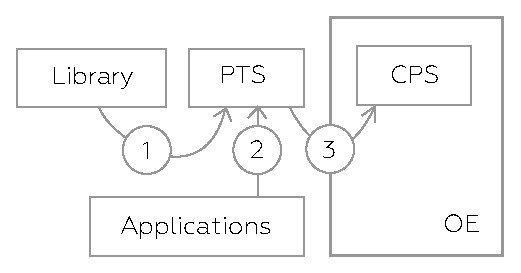
\includegraphics[scale=0.6]{minimal.eps}}
  \caption{Мінімальна система з чистої мови та інтерпретатора}
\end{figure}
\end{center}
Стрілки 1 та 2 визначають
модель та базову бібліотеку, а стрілка 3 означає екстракт
доведення (якщо таке є) в інтерпретатор. Можна використати графічну
мову мереж Петрі для зображення екземпляра моделі системи мов.

\newpage
\subsection{Максимальна система}
Інший приклад системи --- це максимальна система, яка містить усі формальні
мови програмування та формальне середовище виконання (порядок синтаксичних дерев
як параметрів при конструюванні мовної категорії може змінюватися, тут
генеалогія HTS не ведеться від MLTT, яке є розгалуженням).
\begin{equation}
Total =
\begin{cases}
Ob: \{ O_{CPS}, O_{PTS}, O_{MLTT-75}, O_{MLTT-80}, O_{HTS} \} \\
Hom: \begin{cases}
1,2: \mathbb{1} \rightarrow O_{HTS}, 3: O_{MLTT-75} \rightarrow O_{MLTT-80} \\
4: O_{HTS} \rightarrow O_{MLTT-80}, 5: O_{MLTT-80} \rightarrow O_{PTS}, 6: O_{PTS} \rightarrow O_{CPS}
\end{cases}
\end{cases}
\end{equation}
За допомогою мереж Петрі це можна відобразити наступним чином:
\begin{center}
\begin{figure}[ht]
  \centerline{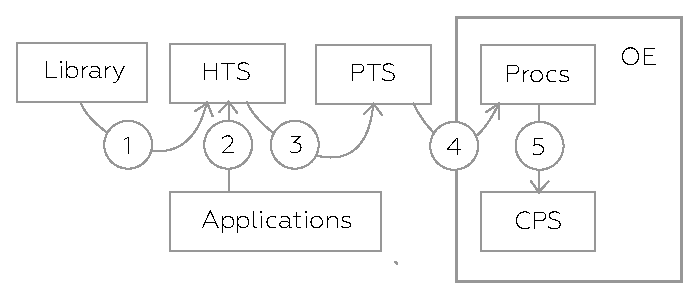
\includegraphics[scale=0.6]{higher.eps}}
  \caption{Кубічна та чиста системи типів та середовище виконання}
\end{figure}
\end{center}


\newpage
\subsection{Категорія середовища виконання CPS}
\begin{definition} (Категорія середовища виконнання $O_{CPS}$).
$$
O_{CPS} =
\begin{cases}
Ob: \{\ maybe\ CPS\ \} \\
Hom: \{\ eval: Ob \rightarrow Ob\ \}
\end{cases}
$$
\end{definition}

Синтаксис середовища виконання може містити наступні синтаксиси:
$O_\lambda$, $O_\pi$, $O_\mu$.

\begin{definition} (Синтаксис мовної категорії $O_{CPS}$).
\begin{lstlisting}
def CPS : U
 := inductive { lambda (c: Joe CPS)
              | process (m: Bob CPS)
              | tensor (f: Alice CPS)
              }
\end{lstlisting}
\end{definition}

Формальне середовище виконання складається з інтерпретатора
(нетитизованого $\lambda$-числення) та числення акторів (процесів, черг, таймерів).
Інтерпретатор та операційна система включені в систему доведення теорем
для уніфікації всіх сигнатур системи та формалізації самого інтерпретатора
як системи виконання. Слід зазначити, що не
завжди є змога зробити екстракт в $O_{CPS}$, тому об'єкти мовних
категорій є $maybe$-типами.
$$
O_{CPS}: O_\lambda \rightarrow O_\pi \rightarrow O_\mu \rightarrow U
$$
Далі буде йтися тільки про формальні інтерпретатори,
так як вони є найбільш компакними формами мов для
верифікації (в порівнянні з моделями System F).
Таким чином будемо розглядати формальне середовище виконання, як
сукупність інтерпретатора та операційної системи.

\begin{definition} (Синтаксичне дерево $O_\lambda$). Інтерпретатор визначається
своїм трьома конструкторами: номер змінної (індекс де Брейна),
лямбда функція та її апплікація:
\begin{lstlisting}
def Joe (cps: U): U
 := inductive { var (x: nat)
              | lam (l: nat) (d: cps)
              | app (f a: cps)
              }
\end{lstlisting}
Мовою інтерпретаторів є нетипизоване лямбда числення, однак в залежності
від складності інтерпретатора це дерево може виглядати по-різному.
\end{definition}

В цьому розділі ми побудуємо надшвидку імплементацію інтерпретатора,
яка цілком, разом зі своїми програмами, розміщується в кеш-памяті
першого рівня процесору, та здатна до AVX векторизацій засобами мови Rust.
Як промислова опція, підтримується також екстракт
в байт-код інтерпретатора BEAM віртуальної машини Erlang.

\begin{definition} (Синтаксичне дерево $O_\pi$).
\begin{lstlisting}
def Bob (lang: U) : U
 := inductive { process (protocol: lang)
              | spawn (cursors: lang) (core: nat) (program: lang)
              | snd (cursor: lang) (data: lang)
              | rcv (cursor: lang)
              | pub (size: nat)
              | sub (cursor: lang)
              }
\end{lstlisting}
\end{definition}

\begin{definition} (Синтаксичне дерево $O_\mu$).
\begin{lstlisting}
def Alice (lang: U) : U
 := inductive { Variable (_: Var)
              | Prim (_: Builtin)
              | Star | True | False
              | Int (_: nat) | Float (_: float)
              | Lambda (a: Var) (b: Linear) (c: Exp)
              | App (a b: Exp)
              | Pair (a b: Var) (c d: Exp)
              | Consume (a: Var) (b c: Exp)
              | Gen (a: Var) (b: Exp)
              | Spec (a: Exp) (b: Fraction)
              | Fix (a b: Var) (c d: Linear) (e: Exp)
              | If (a b c: Exp)
              | Let (a: Var) (b c: Exp)
              }

def Linear : U
 := inductive { Empty | Unit | Bool
              | Int | Float
              | Tensor (a: Fraction) (x: Dimension)
              | Pair (a b: Linear) | Fun (a b: Linear)
              | Consume (a: Linear) | All (a: Var) (b: Linear)
              }

def Builtin : U
 := inductive { Intop (a: Arith) | Floatop (a: Arith)    -- SIMD types
              | Get | Set | Duplicate | Free             -- linearity
              | Transpose | Size                         -- matrices
              | Asum | Axpy | Dotp | Rotm | Scal | Amax  -- BLAS Level 1
              | Symm | Gemm | Syrk | Posv                -- BLAS Level 3
              }

def Fraction  : U := inductive { Z | S (_: Fraction) }
def Dimension : U := inductive { Vector | Matrix | Stream | Table }
def Arith     : U := inductive { Add | Sub | Mul | Div | Eq | Lt | Gt }

\end{lstlisting}
\end{definition}

\newpage
\section{Вищі формальні мови програмування}
Тут йдеться про мови програмування придатні для доведення теорем,
та їх таксономію від найелементарніших (чистої системи з одним типом $\Pi$) до
найпотужніших гомотопічних систем. Одна така гомотопічна система є кінцевим завданням
цього розділу --- побудова моделі гомотопічного верифікатора.
В процесі його побудови в цьому розділі ми розглянемо під
мікроскопом складові частини його нижчих мовних рівнів.

Застосуємо категорну семантику для мов програмування і будемо розглядати
мови програмування як моноїдальні мовні категорі, об'єкти яких є просторами
усіх програм цих мов програмування, а морфізми --- правила верифікації та компіляції цих мов.
Морфізми між мовними категоріями в категорї мов програмування --- це
функтори підвищення та пониження складності мови, подібно до того як діють
морфізми в контекстуальних категоріях. Морфізм деконструює або конструює за
допомогою Either-типу або $\Sigma$-типу індуктивний тип мови програмування.

Мови розкладаються у спектральну (індексовану натуральними числами $N \rightarrow U$)
послідовність мов, кожен елемент якої є мовою програмування,
яка не містить синтаксичне дерево вищої мови програмування.

\newpage
\subsection{Чиста система типів PTS}
Чиста ситема або числення конструкцій або система з одим типом або
система з однією аксіомою, продовжує традиції елементарних пруверів
в стилі першого AUTOMATH та сучасних Henk, Morte, Cedile, Om.

\begin{definition} (Мовна категорія чистої мови $O_{PTS}$).
\begin{equation}
O_{PTS} =
\begin{cases}
Ob: \{\ X: maybe\ PTS, target: maybe\ CPS \ \} \\
Hom: \begin{cases}
type,norm: X \rightarrow X, extract: X \rightarrow target \\
certify: X \rightarrow target = type \circ norm \circ extract
\end{cases}
\end{cases}
\end{equation}
\end{definition}

\begin{definition} (Синтаксис мовної категорії $O_{PTS}$).
Чиста мова $O_{PTS}$ містить лише синтаксис одного типу, $\Pi$-типу.
Така теорія називається теорією з одним типом, або з однією аксіомою.
\begin{lstlisting}
def PTS : U := inductive { forall (_: Pi PTS) }
def Henk := PTS
\end{lstlisting}
\end{definition}

Вона описана в літературі як Calculus of Construction (Кокан),
Pure Type System (Барендрехт, Меєр, Гонзалез, Стемп, Фу).

\begin{definition} (Синтаксичне дерево $O_\Pi$).
\begin{lstlisting}[mathescape=true]
def Pi (lang: U) : U
 := inductive { fibrant (n: nat)
              | variable (x: name) (l: nat)
              | pi (x: name) (l: nat) (f: lang)
              | lambda  (x: name) (l: nat) (f: lang)
              | application (f a: lang)
              }
\end{lstlisting}
\end{definition}

\newpage
\subsection{Теорія типів Мартіна-Льофа MLTT-75$}
Мова теорії типів є сучасною основою всіх пруверів з залежними типами,
такими, наприклад, як NuPRL та Agda. Багато так званих $\Pi\Sigma$ пруверів
імплементують $MLTT-75$ серед таких як:
$\Pi\Sigma$\footnote{\url{https://github.com/zlizta/pisigma-0-2-2}},
$\Pi\forall$\footnote{\url{https://github.com/sweirich/pi-forall}}.

\begin{definition} (Мовна категорія $O_{MLTT-75}$).
\begin{equation}
O_{MLTT-75} =
\begin{cases}
Ob: \{\ maybe\ MLTT-75\ \} \\
Hom: \begin{cases}
type,norm: Ob \rightarrow Ob \\
certify: Ob \rightarrow Ob = type \circ norm
\end{cases}
\end{cases}
\end{equation}
\end{definition}

\begin{definition} (Синтаксис мовної категорії $O_{MLTT-75}$).
Мова $O_{MLTT-75}$ включає в себе синтаксиси трьох типів
теорії Мартіна-Льофа: $O_\Pi$, $O_\Sigma$, $O_=$.
\begin{lstlisting}
def MLTT : U
 := inductive { forall (_: Pi MLTT)
              | sigma (_: Sigma MLTT)
              | id (_: Id MLTT)
              }
\end{lstlisting}
\end{definition}

\begin{definition} (Синтаксичне дерево $O_\Sigma$).
Також можна до чистої системи додати $\Sigma$-тип,
піднявши типову систему до мови $O_{MLTT-72}$ або $O_{\Pi\Sigma}$ :
\begin{lstlisting}[mathescape=true]
def Sigma (lang: U) : U
 := inductive { sigma (n: name) (a b: lang)
              | pair (a b: lang)
              | fst (p: lang)
              | snd (p: lang)
              }
\end{lstlisting}
\end{definition}

\begin{definition} (Синтаксичне дерево $O_=$).
Додавши тип рівності можно підняти систему ще на одну сходинку,
до $O_{MLTT-75}$ або $O_{\Pi\Sigma=}$:
\begin{lstlisting}[mathescape=true]
def Id (lang: U) : U
 := inductive { identity (t a b: lang)
              | id_intro (a b: lang)
              | id_elim (a b c d e: lang)
              | id_compute (a b c d e: lang)
              }
\end{lstlisting}
\end{definition}

$O_=$ не містить $\eta$-правила.

\newpage
\subsection{Система індуктивних типів MLTT-80}

MLTT-80 покладена в основу CCHM верифікатора.

\begin{definition} (Мовна категорія $O_{MLTT-80}$).
\begin{equation}
O_{MLTT-80} =
\begin{cases}
Ob: \{\ X: maybe\ PM, target: maybe\ CPS\ \} \\
Hom: \begin{cases}
type,norm,induction: X \rightarrow X, extract: X \rightarrow target \\
certify : X \rightarrow target \\
cerfity = type \circ norm \circ induction \circ extract \\
\end{cases}
\end{cases}
\end{equation}
\end{definition}

Мова індуктивних типів дозволяє безпосередньо кодувати індуктивні типи,
не використовуючи схеми кодування Бома, містить усі попередні мовні синтаксиси:
$O_=$, $O_\Sigma$, $O_\Pi$ та синтаксиси $O_0$, $O_1$, $O_2$, $O_W$.

\begin{definition} (Синтаксичне дерево мовної категорії $O_{MLTT-80}$).
\begin{lstlisting}
def MLTT-80 := Per
def Per : U
 := inductive { forall (_: Pi Per)
              | sigma (_: Sigma Per)
              | id (_: Id Per)
              | 0 (_: Empty Per)
              | 1 (_: Unit Per)
              | 2 (_: Bool Per)
              | W (_: W Per)
              }

def W (lang: U) : U
 := inductive { W_Form (n: name) (a b: lang)
              | W_Sup (a b: lang)
              | W_Ind (a b c: lang)
              }

def Empty (lang: U) : U := inductive { 0_Ind (a: lang) }
def Unit  (lang: U) : U := inductive { unit | star | 1_Ind (a: lang) }
def Bool  (lang: U) : U := inductive { bool | true | false | 2_Ind (a: lang) }

\end{lstlisting}
\end{definition}

\newpage
\subsection{Система індуктивних типів CIC Paulin-Mohring}

\begin{definition} (Мовна категорія $O_{CIC}$).
\begin{equation}
O_{CIC} =
\begin{cases}
Ob: \{\ X: maybe\ PM, target: maybe\ CPS\ \} \\
Hom: \begin{cases}
type,norm,induction: X \rightarrow X, extract: X \rightarrow target \\
certify : X \rightarrow target \\
cerfity = type \circ norm \circ induction \circ extract \\
\end{cases}
\end{cases}
\end{equation}
\end{definition}

Мова індуктивних типів дозволяє безпосередньо кодувати індуктивні типи,
не використовуючи схеми кодування Бома, містить усі попередні мовні синтаксиси:
$O_=$, $O_\Sigma$, $O_\Pi$.

\begin{definition} (Синтаксичне дерево мовної категорії $O_{CIC}$).

Головним чином, система загальних індуктивних схем предбачає три основних компоненти:
1) верифікатор строго позитивних схем;
2) верифікатор завершуваності рекурсивної перевірки рекурсивних схем;
3) верифікатор взаємної рекурсії.

\begin{lstlisting}
def Frank := := inductive { forall (_: Pi Frank) | inductive (_: Ind Frank) }
def Christine := CIC
def CIC : U
 := inductive { forall (_: Pi CIC)
              | sigma (_: Sigma CIC)
              | id (_: Id CIC)
              | prop (_: Id CIC)
              | inductive (_: Ind CIC)
              }
\end{lstlisting}
\end{definition}

Мова містить наступні допоміжні визначення: i) телескопу,
який містить послідовність елементів мови; ii) розгалуження,
як конструкцій case оператора; iii) імен конструкторів індуктивного типу.

\begin{definition} (Синтаксичне дерево $O_{IND}$).
Правило формації, конструктора та елімінатора визначається синтаксичним деревом $O_{IND}$:
\begin{lstlisting}
def Ind (lang: U) : U
 := inductive { formation (_: Inductive lang)
              | constructor (_: list (triple Nat Inductive lang))
              | eliminator (t: Inductive) (a b: lang) (cases: list lang)
              }

def Inductive (lang: U) : U
 := Σ (name : string)
      (params : list (prod name lang))
      (level : Nat)
      (constrs : list (prod (Nat lang))), 1
\end{lstlisting}
\end{definition}

\newpage
\subsection{Гомотопічна система типів HTS}

Головним чином, гомотопічна система складається з наступних частин:
1) два всесвіти fibrant та pretype;
2) MLTT-75;
3) CCHM розширення.

\begin{definition} (Мовна категорія $O_{HTS}$).
$$
O_{HTS} =
\begin{cases}
Ob: \{\ maybe\ HTS\ \} \\
Hom: \begin{cases}
type,norm: Ob \rightarrow Ob \\
certify: Ob \rightarrow Ob = type \circ norm \\
\end{cases}
\end{cases}
$$
\end{definition}

\begin{definition} (Синтаксис мовної категорії $O_{HTS}$).
Синтаксис гомотопічної мовної категорії містить усі
попередні мовні синтаксиси: $O_I$, $O_W$, $O_=$, $O_\Sigma$, $O_\Pi$:
\begin{lstlisting}
def HTS : U
 := inductive { forall (_: Pi HTS)
              | sigma (_: Sigma HTS)
              | id (_: Id HTS)
              | prop (_: Id HTS)
              | 0 (_: Empty HTS)
              | 1 (_: Unit HTS)
              | 2 (_: Bool HTS)
              | W (_: W HTS)
              | homotopy (_: Homotopy HTS)
              }
\end{lstlisting}
\end{definition}

Гомотопічна типа наслідує $O_{MLTT-80}$ але модифіковану з
Path-типом в індуктивних визначеннях, структурою композиції,
анонсує Path-тип (формація, конструктор, та елімінатор)
як лямбда функцію на відрізку, а також склейку типів у всесвіті
та склейку змінних з відповідними елімінаторами.

\begin{definition} (Синтаксичне дерево $O_I$).
\begin{lstlisting}
def CCHM-CHM (lang: U) : U
 := inductive { pretype (n: nat)
              | PathP (_: lang) | PLam (_: lang) | PApp (f a: lang)
              | I | 0 | 1 | And (a b: lang) | Or (a b: lang) | Neg (_: lang)
              | Transp (a b: lang) | HComp (a b c d: lang)
              | Partial (_: lang) | PartialP (a b: lang) | System (_: lang)
              | Sub (a b c: lang) | Inc (a b: lang) | Ouc (: lang)
              | Glue (: lang) | GlueElem (a b c: lang) | Unglue (_: lang)
              }
\end{lstlisting}
\end{definition}

Таким чином,
$O_{HTS}$ містить два Id-типа, один унаслідований від $O_=$ (з модифікованою
обчислювальною семантикою), а інший Interval який міститься в синтаксичному дереві $O_I$.

\newpage
\section{Висновки}

Таким чином ми здійснили спектралізацію або іншими словами розклали усі
існуючі немодальні формальні системи типів у спектральну категорію.

Системи фібраційного типу Groupoїd Infinity для математичного представлення,
сертифікації (доведення теорем), з екстракцією в сертифікований інтерпретатор
та його середовища виконання.

Основним дослідницьким продуктом є формальне середовище виконання AXIO/1,
яке здатне запускати прості лямбда-програми на верифікованому інтерпретаторі Joe.
Але ніхто не може обмежити розвиток своїх власних вищих мов з екстракцією в цей інтерпретатор.
Метою створення AXIO/1 є утримування процесу розробки під одним авторіті процесі управління
відкритим програмним забезпеченням (Кафедральна модель управління).

AXIO/1 складається з середовища виконання та його мов Joe, Alice, Bob для розробки системного
програмного забезпечення, які використовують стандартний синтаксис ML; і більш високі
мови та їх екстрактори для виконання Alonzo, Henk, Per, Anders для доведення теорем,
які використовують Lean-подібний синтаксис. Неверифікований CPS інтерпретатор реалізований
на мові Rust.


\newpage
\subsection*{Інтерпретатори і системні мови}

Верифікований лямбда-інтерпретатор і паралельне обчислення матриць. Мови Joe,
Bob і Alice мають уніфікований синтаксис Standard ML.

\subsection*{Joe}

Джо є сертифікованим інтерпретатором байт-коду стекової віртуальної машини
та компілятором коду Intel/ARM/SM90.

[1] — MinCaml, [2] — CoqASM. [3] — Verified LISP Interpreter, [4] — Kind, [5] — O-CPS/Rust.

\begin{lstlisting}
fun a (0, n) = n + 1
  | a (m, 0) = a (m - 1, 1)
  | a (m, n) = a (m - 1, a (m, n - 1))
\end{lstlisting}

\subsection*{Bob}

Bob — це паралельне неблокуюче середовище виконання з нульовим копіюванням
та курсорами CAS-кусрорами [4,5] з характеристиками для вбудовуваних систем
реального часу.

[5] — Kernel, [6] — Pony, [7] — Erlang.

\begin{lstlisting}
fun proc =
let val p0 = pub(0,8)
    val s1 = sub(0,p0)
    val s2 = sub(0,p0)
 in send(p0,11);
    send(p0,12);
    [ receive(s1);
      receive(s2);
      receive(s1);
      receive(s2)
    ]
    end
\end{lstlisting}

\subsection*{Alice}

Alice — це числення лінійних типів із частковими дробами [6] для програмування рівня 3 BLAS.

\begin{lstlisting}
fun simpleConvolution (i n: int) (x0: float) (write w: vector float)
  : vector float
  = begin
      if n = i then result.emit(write),
      a = [w0,w1,w2] = w.get(0,3),
      b = [x0,x1,x2] = [ x0 | write.get(i,2) ],
      write.set(i, Dotp(a,b)),
      simpleConvolution((i + 1),n,x1,write,w)
    end
\end{lstlisting}

\newpage
\subsection*{Чисті фібраційні мови програмування (вищих порядків)}

Чисті фібраційні мови мають уніфікований синтаксис Lean-подібної мови.

\subsection*{Alonso}

Alonzo — це система типу STLC-40 як приклад основного числення,
відкритого до фібраційних ΠΣ проверів.

[1] STLC-40 — Проста теорія типів

\begin{lstlisting}
def zero : (T → T) → T → T := λ (s: T → T) (z: T), z
def succ : ((T → T) → T → T) → ((T → T) → T → T)
 := λ (w: (T → T) → T → T) (y: T → T) (x: T), y (w y x)
\end{lstlisting}

\subsection*{Henk}

Henk — це система чистого типу (PTS-91) у стилі числення індуктивних
конструкцій Кокванда/Х’юета (CoC-88) з нескінченною кількістю всесвітів.
Henk також підтримує синтаксис AUTOMATH (AUT-68).

[1] AUT-68 — AUTOMATH 1968, [2] CoC-88 — числення конструкцій, [3] PTS-91 — система чистого типу ($\Pi$).

\begin{lstlisting}
def N := Π (A : U), (A → A) → A → A
def zero : N := λ (A : U) (S : A → A) (Z : A), Z
def succ : N -> N := λ (n : N) (A : U) (S : A → A) (Z : A), S (n A S Z)
def plus (m n : N) : N := λ (A : U) (S : A → A) (Z : A), m A S (n A S Z)
def mult (m n : N) : N := λ (A : U) (S : A → A) (Z : A), m A (n A S) Z
def pow (m n : N) : N := λ (A : U) (S : A → A) (Z : A), n (A → A) (m A) S Z
\end{lstlisting}

\subsection*{Per}

Пер є $\Pi\Sigma$ (MLTT-72) прувером із численням індуктивних конструкцій
та типами тотожності (MLTT-75). Природне розширення CoC до CIC було
зроблено Франком Пфеннінгом і Крістін Полін (IND-89).

[1] Mini-TT — реалізація OCaml,
[2] MLTT-72 — Пі, Sigma,
[3] MLTT-75 — Pi, Sigma, Id,
[4] MLTT-80 — 0, 1, 2, W, Pi, Sigma, Id,
[5] PP-89 — Індуктивно визначені типи,
[6] CIC-2015 — Числення індуктивних конструкцій.

\begin{lstlisting}
def empty      : U := inductive { }
def L¹ (A : U) : U := inductive { nil | cons (head: A) (tail: L¹ A) }
def S¹         : U := inductive { base | loop : Equ S¹ base base }

def quot (A: U) (R : A -> A -> U) : U
 := inductive { quotient (a: A)
              | identification (a b: A) (r: R a b)
              : Equ (quot A R) (quotient a) (quotient b)
              }
\end{lstlisting}
\\
\\
\newpage
\subsection*{Anders}

Anders — це система гомотопічних типів (HTS-2013) із примітивами суворої рівності та кубічної Agda (CCHM-2016).

[1] HTS-2013 — система гомотопічних типів,
[2] BCH-2014 — Кубічні набори,
[3] CCHM-2015 — Система кубічного типу,
[4] ОП-2016 — Топосні аксіоми,
[5] CHM-2017 — Рівняння Губера,
[6] ВМА-2017 — Кубічна Агда.

\begin{lstlisting}
def idfun  (A : U) : A $\rightarrow$ A := ($\lambda$ (a : A), a
def idfun' (A : U) : A $\rightarrow$ A := transp (<i> A) 0
def idfun'' (A : U) : A $\rightarrow$ A := ($\lambda$ (a : A), hcomp A 0 ($\lambda$ (i : I), []) a
def isFiberBundle (B: U) (p: B $\rightarrow$ U) (F: U): U
 := Σ (v: U) (w: surjective v B), (Π (x: v), PathP (<_>U) (p (w.1 x)) F)
def ~~ (X : U) (a x' : X) : U := Path ($\Im$ X) ($\iota$ X a) ($\iota$ X x')
def $\mathbb{D}$ (X : U) (a : X) : U := Σ (x′ : X), ~~ X a x'
def unitDisc (X : U) (x : $\Im$ X) : U := Σ (x' : X), Path ($\Im$ X) x ($\iota$ X x')
def starDisc (X : U) (x : X) : $\mathbb{D}$ X x := (x, idp ($\Im$ X) ($\iota$ X x))
def T$^\infty$ (A : U) : U := Σ (a : A), $\mathbb{D}$ A a
def inf-prox-ap (X Y : U) (f : X $\rightarrow$ Y) (x x' : X) (p : ~~ X x x')
  : ~~ Y (f x) (f x') := <i> $\Im$-app X Y f (p @ i)
def d (X Y : U) (f : X $\rightarrow$ Y) (x : X) ($\epsilon$ : $\mathbb{D}$ X x) : $\mathbb{D}$ Y (f x)
 := (f $\epsilon$.1, inf-prox-ap X Y f x $\epsilon$.1 $\epsilon$.2)
def T$^\infty$-map (X Y : U) (f : X $\rightarrow$ Y) ($\tau$ : T$^\infty$ X) : T$^\infty$ Y
 := (f $\tau$.1, d X Y f $\tau$.1 $\tau$.2)
def is-homogeneous (A : U)
 := Σ (e : A) (t : A $\rightarrow$ equiv A A),
    Π (x : A), Path A ((t x).1 e) x
\end{lstlisting}

\subsection*{Urs}

Urs — це еквіваріантна система супергомотопічних типів з ферміонними та бозонними модальностями,
вбудованими в верифікатор.

[1] R-HoTT — Rezk Infinity Categories,
[2] G-HoTT — Guarded Cubical,
[3] L-HoTT — Linear HoTT,
[4] ES-HoTT — Equivariant Super HoTT.

